\documentclass[10pt,a4paper]{article}
\usepackage[margin=20mm]{geometry}
\usepackage[T1]{fontenc}
\usepackage{lmodern,microtype,amsmath,amssymb,booktabs,graphicx,siunitx,tikz}
\usepackage[hidelinks]{hyperref}
\hypersetup{pdftitle={Space-charge fields of straight and curved long bunches},
pdfsubject={OPALX 2D5, curvature correction, SACR and PyORBIT comparisons}}
\usepackage{etoolbox}
\usepackage{float}
\usepackage[section]{placeins}
\BeforeBeginEnvironment{figure}{\par}
\AfterEndEnvironment{figure}{\par}
\BeforeBeginEnvironment{table}{\par}
\AfterEndEnvironment{table}{\par}
\usepackage[font=small,labelfont=bf]{caption}
\usetikzlibrary{arrows.meta,positioning,calc,decorations.markings}
\setlength{\parindent}{0pt}
\setlength{\parskip}{4pt}
\setlength{\textfloatsep}{11pt}
\setlength{\floatsep}{9pt}
\clubpenalty=10000
\widowpenalty=10000
\newcommand{\dd}{\mathrm d}
\newcommand{\eps}{\epsilon_0}
\newcommand{\kC}{k_{\mathrm e}}
\newcommand{\er}{\mathbf e_u}
\newcommand{\es}{\mathbf e_s}
\newcommand{\ey}{\mathbf e_y}
\newcommand{\figfile}[2]{\IfFileExists{figures/#1}{\includegraphics[width=#2\linewidth]{figures/#1}}{}}
\title{Space-charge fields of straight and curved long bunches\\[3pt]
\large Original and corrected OPALX 2D5, SACR and PyORBIT}
\author{}
\date{}
\begin{document}
\maketitle
\vspace{-2.5em}
\begin{abstract}
We compare frozen space-charge fields for a \SI{5}{m} bunch carrying
\SI{10}{pC}, with nominal \SI{10}{mm} rms size in each transverse direction.
Straight and \SI{2}{m}-radius sources share uniform round cross-sections
and either uniform or triangular longitudinal profiles. The comparison
separates the original transverse-slice model, its first-order curvature
extension, an independent Coulomb reference, and the matched PyORBIT model.
\IfFileExists{results/abstract.tex}{The transverse curvature correction recovers the outward centre field; the local longitudinal models retain finite-source errors already visible in the straight bunch.
}{}
\IfFileExists{results/tracking-abstract.tex}{Ten-step native tracking comparisons test the original slice models with matched-source ZeroSC controls.
}{}
\end{abstract}

\section{Common charge distribution}
The transverse density is uniform inside a disk of radius
$a=\SI{20}{mm}$, corresponding to $\sigma_x=\sigma_y=\SI{10}{mm}$ in the
straight case. The curved case uses the same physical cross-section.
Let $u$ and $y$ denote the local
transverse coordinates, and let $s$ measure arclength from the bunch centre.
The physical volume density is
\begin{equation}
 \rho(u,y,s)=\frac{\lambda(s)}{\pi a^2}\,
 \mathbf 1_{u^2+y^2<a^2},\qquad
 \lambda_{\rm U}(s)=\frac{Q}{L},\qquad
 \lambda_{\rm T}(s)=\frac{2Q}{L}\left(1-\frac{2|s|}{L}\right),
 \label{eq:source}
\end{equation}
for $|s|<L/2$, and zero outside. Here $Q=\SI{10}{pC}$ and
$L=\SI{5}{m}$. In the straight case $u=x$. The circular source has
\begin{equation}
 \mathbf X(u,y,s)=\bigl((R+u)\cos(s/R)-R,\ y,\ (R+u)\sin(s/R)\bigr),
 \qquad J=1+u/R,\qquad \dd V=J\,\dd u\,\dd y\,\dd s.
 \label{eq:map}
\end{equation}
Positive $u$ points outward. All models use the same physical source,
charge and free-space boundary condition; no conducting pipe is present.
The frozen-field tests use protons at $\beta=10^{-3}$ and one field
evaluation. Fields are reported in the electrostatic convention.
We remove the native longitudinal $\gamma^{-2}$ factor before comparison.
The longitudinal numerical periods are \SI{12}{m} for the straight source
and the reference circumference for the circular source. Each contains
one \SI{5}{m} bunch and a vacuum gap; SACR includes no periodic images.
\begin{figure}[ht]
\centering
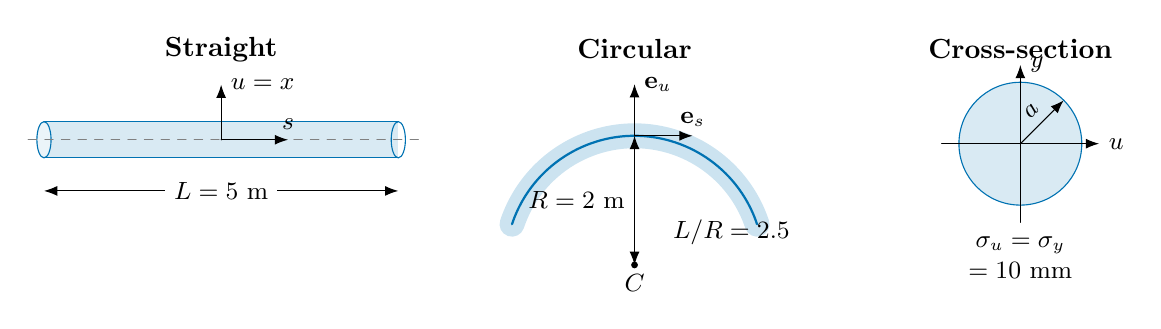
\begin{tikzpicture}[>=Latex,font=\small,line cap=round,line join=round]
\definecolor{beam}{RGB}{0,114,178}
\begin{scope}[shift={(0,0)}]
 \node[font=\bfseries] at (2.25,1.15) {Straight};
 \fill[beam!15] (0,-.23) rectangle (4.5,.23);
 \draw[beam] (0,-.23)--(4.5,-.23) (0,.23)--(4.5,.23);
 \draw[beam,fill=beam!8] (0,0) ellipse (.09 and .23);
 \draw[beam] (4.5,0) ellipse (.09 and .23);
 \draw[dashed,gray] (-.2,0)--(4.8,0);
 \draw[<->] (0,-.65)--node[fill=white] {$L=5$ m}(4.5,-.65);
 \draw[->] (2.25,0)--(3.1,0) node[above] {$s$};
 \draw[->] (2.25,0)--(2.25,.7) node[right] {$u=x$};
\end{scope}
\begin{scope}[shift={(7.5,.05)},scale=.82]
 \node[font=\bfseries] at (0,1.34) {Circular};
 \draw[beam!20,line width=9pt] (0,-2) ++(161.6197:2)
   arc[start angle=161.6197,end angle=18.3803,radius=2];
 \draw[beam,thick] (0,-2) ++(161.6197:2)
   arc[start angle=161.6197,end angle=18.3803,radius=2];
 \fill (0,-2) circle (1.5pt) node[below] {$C$};
 \draw[<->] (0,-2)--node[left] {$R=2$ m}(0,0);
 \draw[->] (0,0)--(.9,0) node[above] {$\mathbf e_s$};
 \draw[->] (0,0)--(0,.8) node[right] {$\mathbf e_u$};
 \node at (1.5,-1.5) {$L/R=2.5$};
\end{scope}
\begin{scope}[shift={(12.4,-.05)}]
 \node[font=\bfseries] at (0,1.2) {Cross-section};
 \fill[beam!15] (0,0) circle (.78);
 \draw[beam] (0,0) circle (.78);
 \draw[->] (-1,0)--(1,0) node[right] {$u$};
 \draw[->] (0,-1)--(0,1) node[right] {$y$};
 \draw[->] (0,0)--node[above,sloped] {$a$}(.55,.55);
 \node[align=center] at (0,-1.45) {$\sigma_u=\sigma_y$\\$=10$ mm};
\end{scope}
\end{tikzpicture}

\caption{Common source geometry: straight cylinder, circular tube and local
cross-section. The bunch length is \SI{5}{m}; the transverse radius is
\SI{20}{mm}, giving nominal \SI{10}{mm} rms sizes. Tube thickness is exaggerated
in the side views. The bending radius is \SI{2}{m}; the charged arc subtends
$L/R=2.5$ rad.}
\label{fig:geometry}
\end{figure}
\IfFileExists{results/source.tex}{\begin{figure}[!ht]\centering
\includegraphics[width=\linewidth]{figures/charge-distribution.pdf}
\caption{Common physical source and charge marginals. Lines describe the
prescribed density; circles and squares are histograms of the shared
straight and curved particle sources. All native models use the same
source files within each geometry. The small curved radial asymmetry is
the volume factor $J$; it does not change the physical disk radius.}
\label{fig:source}\end{figure}
Each frozen-field native case uses $8\,388\,608$ equal-charge source particles. The
transverse numerical box is $48\times48$ mm. We compare
$128^2\times512$ and $256^2\times1024$ meshes with the same source;
these test two resolutions rather than establish asymptotic convergence.
}{}

\section{Field models}
\subsection{Original OPALX 2D5}
The original model solves one free-space transverse Poisson equation per
longitudinal slice and adds a local longitudinal field,
\begin{equation}
 \nabla_\perp^2\Phi_c=-\rho_c/\eps,\qquad
 \mathbf E_\perp=-\nabla_\perp\Phi_c,\qquad
 E_s=-\frac{g}{4\pi\eps\gamma^2}\frac{\dd\lambda}{\dd s},
 \label{eq:original}
\end{equation}
where $\rho_c=\dd q/(\dd u\dd y\dd s)=J\rho$ is the deposited coordinate
density. We retain the prescribed $g=6.36$ to match the original model,
without fitting it to the finite bunch. This local closure belongs to the
line-density-derivative family discussed in Ref.~\cite{oeftiger}.
The reference path and particle containers share one spatial solve frame.
The transverse solver uses the rectangular-cell averaged logarithmic
Green function and centred potential gradients.

\subsection{Corrections and curvature extension}
The earlier numerical fixes correct field normalization, the magnetic-field
orientation, frame consistency, endpoint coverage and the transverse
self-cell integral. The additional curvature model described here changes
the transverse field approximation. Long-bunch curvature corrections have
also been studied by Qiang~\cite{qiang}; the construction below follows a
direct expansion of Coulomb's law for this comparison.

Write $\kappa=1/R$, let primed coordinates refer to the source, and let
$D=|\mathbf X-\mathbf X'|$ be the physical source--target distance. Define
$\xi=2\sin[\kappa(s'-s)/2]/\kappa$ and
$D_0^2=(u-u')^2+(y-y')^2+\xi^2$. To first order in transverse offset/R,
\begin{equation}
 \frac{J'}{D}=\frac{1}{D_0}+\kappa\left[
 \frac{u'}{D_0}-\frac{(u+u')\xi^2}{2D_0^3}\right]+\cdots.
 \label{eq:expansion}
\end{equation}
This produces an auxiliary source $u'\rho$, a radial-position-weighted
moment of the existing density. Dividing $\rho_c$ by $J$ recovers the
physical density used in the two ordinary 2D solves,
\begin{equation}
 \Phi_0=G_{2\mathrm D}*\rho,\qquad
 \Phi_u=G_{2\mathrm D}*(u'\rho),\qquad
 G_{2\mathrm D}(r)=-2\kC\log(r/r_0),\quad
 \kC=\frac{1}{4\pi\eps}.
\end{equation}
The matched transverse potential is
\begin{equation}
 \Phi_\perp=\Phi_0+\frac{\kappa}{2}(\Phi_u-u\Phi_0)
                  +\kC\kappa\lambda u-uC(s),\qquad
 (E_u,E_y)=-\nabla_\perp\Phi_\perp,
 \label{eq:correction}
\end{equation}
where $C$ is the finite-part circular line integral,
\begin{equation}
 C(s)=\kC\lim_{h\to0}\left[
 \int_{|\delta|>h}\frac{\kappa|\kappa|\lambda(s+\delta)}
 {4|\sin(\kappa\delta/2)|}\,\dd\delta
 +\kappa\lambda(s)\log(2h/r_0)\right].
 \label{eq:line}
\end{equation}
The matching distance $h$ and logarithmic reference length $r_0$ cancel.
The algorithm uses two transverse FFT solves and one 1D line integral,
with no 3D FFT. It retains the local longitudinal closure in
Eq.~\eqref{eq:original}. The approximation assumes a thin tube and slow
longitudinal variation on the transverse scale. At $\kappa=0$, the
curvature-corrected slice model equals the original model exactly.

\subsection{Semi-analytic curved-tube reference (SACR)}
SACR evaluates the electrostatic field of the prescribed finite charge
volume $V$ in free space. With $D=|\mathbf X_t-\mathbf X'|$ and
$\dd V'=J'\dd u'\dd y'\dd s'$, Coulomb's law gives
\begin{align}
 \Phi(\mathbf X_t)&=\kC\int_V\frac{\rho(\mathbf X')}{D}\,\dd V',
 \qquad \Phi\to0\quad\text{as }|\mathbf X_t|\to\infty,\\
 \mathbf E(\mathbf X_t)&=\kC\int_V\rho(\mathbf X')
 \frac{\mathbf X_t-\mathbf X'}{D^3}\,\dd V'.
 \label{eq:sacr}
\end{align}
The exact curved distance and volume factor are retained. The tube marks
where charge is present; the field occupies all space. The straight
source--target chord may leave the tube and cross uncharged vacuum
(Fig.~\ref{fig:sacr}). The kernel uses its Euclidean length, with no
visibility restriction. There is no conducting beam pipe, induced wall
charge or periodic Coulomb image.

To integrate by parts, differentiate with respect to the Cartesian source
position, keeping the target fixed:
\begin{align}
 \nabla' D^{-1}&=\frac{\mathbf X_t-\mathbf X'}{D^3},\\
 \rho\nabla' D^{-1}&=\nabla'\!\left(\frac{\rho}{D}\right)
                      -\frac{\nabla'\rho}{D}.
\end{align}
Integrating this product rule over $V$ and applying the divergence theorem
component by component yields
\begin{equation}
 \frac{\mathbf E}{\kC}
 =\int_V\nabla'\!\left(\frac{\rho}{D}\right)\dd V'
  -\int_V\frac{\nabla'\rho}{D}\,\dd V'
 =\oint_{\partial V}\frac{\rho\,\mathbf n'}{D}\,\dd S'
  -\int_V\frac{\nabla'\rho}{D}\,\dd V'.
 \label{eq:sacr-surface}
\end{equation}
Here $\mathbf n'$ points out of the charge volume. For an interior target,
exclude a small sphere about $\mathbf X_t$ before taking the limit; its
surface contribution vanishes as the sphere shrinks. The surface formula
is an exact rewriting of the volume field, without extra physical surface
charge. Density jumps at the outer boundary are represented by its surface
term; $\nabla'\rho$ denotes the gradient inside $V$.

For the constant-radius tube, write $b=L/2$ and
$A=\{(u',y'):u'^2+y'^2<a^2\}$. Its boundary consists of the curved side
and two planar disks,
\begin{equation}
 S_\pm=\{\mathbf X(u',y',\pm b):(u',y')\in A\},\qquad
 \mathbf n'_\pm=\pm\mathbf e_s(\pm b),\qquad
 \dd S'=\dd u'\dd y'.
 \label{eq:cap-geometry}
\end{equation}
These \emph{end caps} close the charge volume where the bunch stops.
They are not electrodes or imposed potential boundaries. Their normals
follow the local tangent, so the two cap planes are not parallel in a bend.
If $\rho_\pm$ are the density limits approached from inside the bunch,
their contribution to the surface representation is
\begin{equation}
 \mathbf E_{\rm caps}=\kC\sum_{\sigma=\pm1}
 \sigma\rho_\sigma\,\mathbf e_s(\sigma b)
 \int_A\frac{\dd u'\dd y'}
 {|\mathbf X_t-\mathbf X(u',y',\sigma b)|}.
 \label{eq:cap-field}
\end{equation}
Uniform density has $\nabla'\rho=0$ inside: the curved side and both caps
supply the complete field. For the triangular profile, $\rho_\pm=0$, so
the caps contribute zero, while the side and interior gradient remain.
These terms still include the finite-end field.
In physical curved coordinates this gradient is
\begin{equation}
 \nabla'\rho=\frac{\mathbf e_s(s')}{J'}
             \frac{\lambda'(s')}{\pi a^2}.
 \label{eq:sacr-gradient}
\end{equation}
The factor $1/J'$ cancels the volume Jacobian in the gradient integral.
The continuous triangular cusp at $s'=0$ changes the slope but adds no
surface term. Analytic longitudinal primitives and converged geometric
quadrature evaluate the remaining integrals; target-centred quadrature
resolves the integrable singularity without softening.
\begin{figure}[ht]
\centering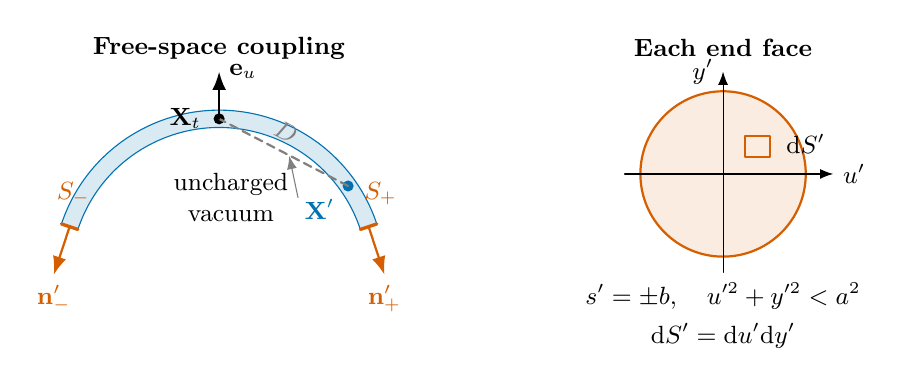
\begin{tikzpicture}[>=Latex,font=\small,line cap=round,line join=round]
\definecolor{sacrblue}{RGB}{0,114,178}
\definecolor{caporange}{RGB}{213,94,0}
\begin{scope}[shift={(2.5,1.6)}]
 \node at (0,.9) {\textbf{Free-space coupling}};
 \fill[sacrblue!15] (0,-2) ++(161.62:2.11)
   arc[start angle=161.62,end angle=18.38,radius=2.11]
   -- ++(198.38:.22)
   arc[start angle=18.38,end angle=161.62,radius=1.89] -- cycle;
 \draw[sacrblue] (0,-2) ++(161.62:1.89)
   arc[start angle=161.62,end angle=18.38,radius=1.89];
 \draw[sacrblue] (0,-2) ++(161.62:2.11)
   arc[start angle=161.62,end angle=18.38,radius=2.11];
 \draw[caporange,very thick] (0,-2) ++(161.62:1.89)--++(161.62:.22);
 \draw[caporange,very thick] (0,-2) ++(18.38:1.89)--++(18.38:.22);
 \coordinate (target) at (0,0);
 \coordinate (source) at (1.638,-.853);
 \fill[sacrblue] (source) circle (2pt) node[below left=2pt] {$\mathbf X'$};
 \fill (target) circle (2pt) node[left=3pt] {$\mathbf X_t$};
 \draw[densely dashed,gray,thick] (source)--node[above,sloped,pos=.55] {$D$}(target);
 \node[align=center] (vacuum) at (.15,-1.0) {uncharged\\vacuum};
 \draw[->,gray] (vacuum.east)--(.89,-.47);
 \draw[->,thick] (target)--(0,.6) node[right] {$\mathbf e_u$};
 \draw[->,caporange,thick] (-1.898,-1.369)--(-2.10,-1.98)
   node[below] {$\mathbf n'_-$};
 \draw[->,caporange,thick] (1.898,-1.369)--(2.10,-1.98)
   node[below] {$\mathbf n'_+$};
 \node[caporange] at (-1.85,-.95) {$S_-$};
 \node[caporange] at (2.05,-.95) {$S_+$};
\end{scope}
\begin{scope}[shift={(8.9,.9)}]
 \node at (0,1.6) {\textbf{Each end face}};
 \filldraw[fill=caporange!12,draw=caporange,thick] (0,0) circle (1.05);
 \draw[->] (-1.25,0)--(1.4,0) node[right] {$u'$};
 \draw[->] (0,-1.25)--(0,1.3) node[left] {$y'$};
 \draw[caporange,thick] (.28,.22) rectangle (.60,.48);
 \node[anchor=west] at (.68,.38) {$\dd S'$};
 \node[align=center] at (0,-1.8)
   {$s'=\pm b,\quad u'^2+y'^2<a^2$\\[3pt]
    $\dd S'=\dd u'\dd y'$};
\end{scope}
\end{tikzpicture}

\caption{Free-space SACR geometry. The dashed Coulomb chord can pass outside
the charged tube; the uncharged region does not screen the interaction.
Orange marks the two end faces of the charge volume. Each is a disk normal
to its local reference tangent, with outward normal
$\mathbf n'_\pm=\pm\mathbf e_s(\pm b)$. These faces are not conducting plates.
The right panel shows their common cross-section. Tube thickness is exaggerated.}
\label{fig:sacr}
\end{figure}

The first SACR verification used a different source: a bent,
uniform-density ellipsoid with tapered semiaxes
\begin{equation}
 a(s)=a_0\sqrt{1-s^2/b^2},\qquad
 c(s)=c_0\sqrt{1-s^2/b^2},\qquad
 \lambda_{\rm E}(s)=\frac{3Q}{4b}\left(1-\frac{s^2}{b^2}\right).
 \label{eq:sacr-ellipsoid}
\end{equation}
At fixed $a_0,b,c_0,Q$, $R\to\infty$ gives Dubin's Cartesian uniform
ellipsoid~\cite{dubin}. Its cross-section shrinks to a point at each end;
there are no finite-area planar caps. This paper instead keeps radius $a$
constant and prescribes uniform or triangular line density. The same SACR
Coulomb method applies, but its straight limit is the corresponding finite
cylinder, not the ellipsoid. Changing the line density inside a fixed
cylinder is different from tapering its cross-section.

\begin{samepage}
Independent Cartesian volume integration and scalar-potential differences
check the field, alongside reflection symmetries, Gauss's law and the
straight-radius limit. The current uniform-cylinder axis has the exact
charged-disk check~\cite{disk},
\begin{equation}
 E_s(0,0,s)=\frac{\rho_0}{2\eps}\left[
 2s+\sqrt{(b-s)^2+a^2}-\sqrt{(b+s)^2+a^2}\right],\qquad |s|<b,
 \label{eq:axis}
\end{equation}
where $\rho_0=Q/(\pi a^2L)$. These checks keep the reference independent of
the original and corrected slice approximations.
\end{samepage}

\subsection{PyORBIT model used here}
We use PyORBIT's native \texttt{SpaceChargeCalcSliceBySlice2D} without a
conducting boundary, together with \texttt{LSpaceChargeCalc} in gradient
mode~\cite{pyorbit,pyorbitcode}. It supplies independent transverse slice
fields and the same prescribed $g=6.36$ longitudinal closure. The constructor
ratio encodes this coefficient only; it does not introduce a physical pipe.
Source coordinates, particle charges, mesh spacing and longitudinal period
match original OPALX. Both use the reference polyline; corrected OPALX
uses the same Cartesian particles with exact-circle coordinates and period.
These standard PyORBIT modules contain no circular Coulomb coupling.

\begin{figure}[ht]
\centering
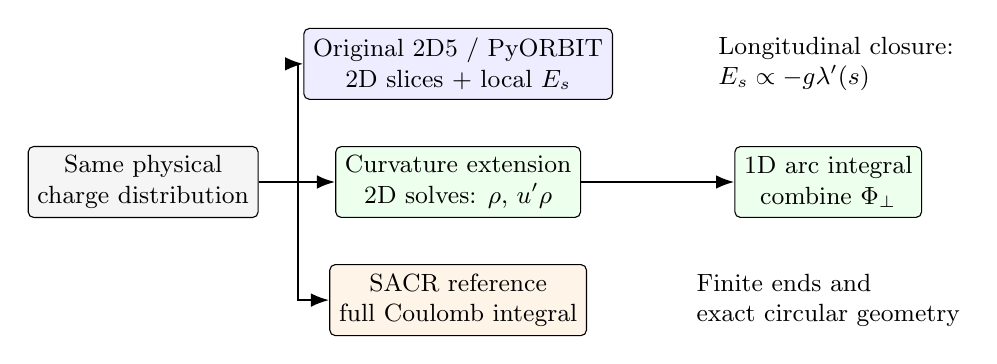
\begin{tikzpicture}[>=Latex,font=\small,
 box/.style={draw,rounded corners=2pt,minimum height=9mm,align=center},
 arrow/.style={->,thick}]
 \node[box,fill=gray!8] (source) at (0,0) {Same physical\\charge distribution};
 \node[box,fill=blue!7] (old) at (4,1.5) {Original 2D5 / PyORBIT\\2D slices + local $E_s$};
 \node[box,fill=green!7] (fix) at (4,0) {Curvature extension\\2D solves: $\rho$, $u'\rho$};
 \node[box,fill=green!7] (line) at (8.7,0) {1D arc integral\\combine $\Phi_\perp$};
 \node[box,fill=orange!9] (sacr) at (4,-1.5) {SACR reference\\full Coulomb integral};
 \draw[arrow] (source.east)--++(.5,0)|-(old.west);
 \draw[arrow] (source.east)--(fix.west);
 \draw[arrow] (source.east)--++(.5,0)|-(sacr.west);
 \draw[arrow] (fix.east)--(line.west);
 \node[align=left] at (8.8,1.5) {Longitudinal closure:\\$E_s\propto-g\lambda'(s)$};
 \node[align=left] at (8.7,-1.5) {Finite ends and\\exact circular geometry};
\end{tikzpicture}

\caption{The model operations. All branches start from the same source.
The auxiliary $u'\rho$ is a mathematical moment, not additional physical
charge. SACR integrates the full curved source; the corrected slice model
adds its first-order transverse curvature contribution.}
\label{fig:models}
\end{figure}

\section{Independent validation of SACR}
The reference is checked directly for the current constant-radius tube.
A separate implementation integrates the original Cartesian Coulomb vector
with the physical volume factor $J$, without surface formulas, softening or
charge renormalization. Eight targets per profile include mixed transverse
bulk points, off-axis points 10 and 5 mm from an end, and an axis point
0.1 mm from an end. Five targets per profile have all three field components
nonzero. Angular and radial refinements are independent of the SACR rule.
\begin{figure}[!ht]\centering
\includegraphics[width=\linewidth]{figures/sacr-volume-validation.pdf}
\caption{Independent volume integration versus SACR for both profiles and
all three field components. Lower panels retain signed differences; bars
show the change under the final volume-rule refinement, not a statistical
confidence interval. Probe indices are centre (1), bulk (2--3), off-axis
10 mm from the end (4--5), axis 5 mm and 0.1 mm from the end (6--7), and
off-axis 5 mm from the end (8). All axes include zero.}
\label{fig:sacr-volume-validation}\end{figure}
The largest observed difference among 48 components is $2.2\times10^{-11}$ V/m; the final independent refinement changes a component by at most $1.5\times10^{-10}$ V/m. These are sampled numerical checks rather than a uniform error bound.

\begin{samepage}
A second check keeps charge, tube cross-section, line-density profile and
15 material targets fixed while increasing $R$ from 2 to 1000 m. The same
curved SACR implementation also evaluates $R=\infty$ and is compared with
the separately derived finite-cylinder reference. Define
\begin{equation}
 \Delta_i(R)=\frac{\max_{15\ {\rm targets}}
 |E_i^{\rm SACR}(R)-E_i^{\rm cylinder}|}{E_{i,*}},\qquad
 E_{i,*}=\max_{51\ {\rm straight\ targets}}|E_i^{\rm cylinder}|.
\end{equation}
The fixed component scale retains targets with zero field. Finite-radius
differences measure the physical change in source geometry.
\end{samepage}
\begin{figure}[!ht]\centering
\includegraphics[width=\linewidth]{figures/sacr-radius-convergence.pdf}
\caption{Constant-section SACR approaches the straight-cylinder field as
curvature tends to zero. Each point is the maximum difference over the same
15 material targets, divided by its fixed straight component scale.
Both axes retain zero; the point at $1/R=0$ is an actual infinite-radius
calculation. These geometry differences are distinct from quadrature error.}
\label{fig:sacr-radius-convergence}\end{figure}
The straight-limit implementations differ by at most $6.9\times10^{-15}$ V/m over the selected targets. The largest recorded radius-sweep quadrature change is $3.8\times10^{-15}$ V/m. The two checks support using SACR as the independent frozen-field reference for this tube; they do not validate beam tracking.


\section{Straight-bunch comparison}
We first set $\kappa=0$. Original 2D5 and its curvature-corrected slice
limit coincide, so one native slice result represents both. The separate
straight finite-source 3D FFT branch is excluded from this comparison.
Equal-charge sources and matched probe-only companions remove diagnostic
particle fields. Numerical source, mesh and reference errors are checked
separately. Signed field and residual axes include zero.
\IfFileExists{results/straight.tex}{\begin{figure}[!ht]
\centering\includegraphics[width=\linewidth]{figures/straight-fields.pdf}
\caption{Straight-bunch fields for uniform (upper rows) and triangular
(lower rows) profiles. Transverse cuts pass through the centre; the
longitudinal cut follows the positive axis and uses logarithmic distance
to the end. Lower panels show native minus finite-source reference.
The original and curvature-corrected slice models coincide at zero curvature.
All field axes retain zero.}\label{fig:straight-fields}\end{figure}
The straight triangular bunch already exposes the longitudinal limitation: at $s=1.25$ m, the local models give $0.09146$ V/m, versus $0.13745$ V/m from the finite-source reference (33.5\% low). For the uniform bunch, the local derivative vanishes in the interior although the finite-source end field remains nonzero. Refining the numerical end stencil cannot supply that nonlocal tail.
The symmetric particle rule removes artificial $x/y$ anisotropy at fixed particle count. Residual point-kernel/source sampling errors remain, especially in PyORBIT; the two meshes do not establish monotonic convergence.
}{}

\section{Circular-bunch comparison}
The second case uses the same physical density with $R=\SI{2}{m}$.
The curvature-corrected OPALX run uses Eq.~\eqref{eq:correction}; original
OPALX and PyORBIT retain their slice approximations. We compare the centre
radial field separately from the much larger transverse field gradient.
\IfFileExists{results/curved.tex}{\begin{figure}[!ht]
\centering\includegraphics[width=\linewidth]{figures/curved-fields.pdf}
\caption{Circular-bunch fields for the same source at $R=2$ m, with the
same cuts and residual convention as Fig.~\ref{fig:straight-fields}.
The correction changes the transverse field; its longitudinal field still
uses the local $g=6.36$ closure.}\label{fig:curved-fields}\end{figure}
\FloatBarrier
\begin{figure}[H]
\centering\includegraphics[width=\linewidth]{figures/curved-even-field.pdf}
\caption{Weak radial curvature field, isolated as
$[E_u(+u)+E_u(-u)]/2$ at $y=s=0$. The two meshes are shown separately;
the zero line is retained.}\label{fig:even}\end{figure}
\begin{table}[!ht]\centering\small\caption{Centre radial field in V/m; positive is outward.}\begin{tabular}{llrr}\toprule Profile&Model&$128^2\!\times512$&$256^2\!\times1024$\\\midrule
Uniform&Original 2D5&-0.009000&-0.008949\\
Uniform&Corrected 2D5&+0.040925&+0.040929\\
Uniform&PyORBIT&-0.009102&-0.008310\\
&SACR&+0.040936&+0.040936\\
\addlinespace
Triangle&Original 2D5&-0.017909&-0.017853\\
Triangle&Corrected 2D5&+0.063607&+0.063576\\
Triangle&PyORBIT&-0.018231&-0.016493\\
&SACR&+0.063687&+0.063687\\
\bottomrule\end{tabular}\label{tab:centre}\end{table}
The corrected centre fields agree with SACR within 0.18\% on both meshes. Across the sampled midplane pairs, the weak-field relative errors stay below 0.68\%. The original model and matched PyORBIT retain the inward centre field. The correction repairs this transverse curvature contribution; the longitudinal discrepancy persists.
}{}

\section{First native tracking comparison}
The first tracking case uses the uniform longitudinal profile and the same
physical disk and length, sampled by $1\,048\,576$ equal-charge particles.
Each geometry shares identical initial particle coordinates and momenta
between the codes. Cold protons at $\beta=10^{-3}$ advance a nominal 1 m in
exactly ten midpoint steps, $\Delta t=\SI{0.333564}{\micro s}$.
A ZeroSC companion keeps the same nominal charge and particle mass while
disabling self-fields. We compare both total centred RMS sizes and
$\Delta\sigma_i=\sigma_i(10\,\mathrm{pC})-\sigma_i(\mathrm{ZeroSC})$.

OPALX uses the original slice baseline, not the transverse curvature
extension. PyORBIT uses its native drift and sector-bend body maps with
native transverse slices and local longitudinal kicks. Both retain the
physical $g=6.36$; PyORBIT's per-turn longitudinal normalization is scaled
by step length divided by numerical period. The grid is
$128^2\times512$ in a 48 mm transverse box. The straight numerical period
is 12 m; the bend uses the common reference-polyline circumference.
The transverse PyORBIT kick retains its native approximation of omitting
transverse work from its energy coordinate.

\begin{figure}[!ht]\centering
\includegraphics[width=\linewidth]{figures/tracking-comparison.pdf}
\caption{Exactly ten native tracking steps per case, with a same-source
ZeroSC companion. Upper rows show centred RMS sizes; lower rows isolate
the self-field response. Straight $u=x$; bend $u,y,s$ are local circular
coordinates, rather than whole-bunch Cartesian projections. The horizontal
axis is nominal central-particle flight. All size and response axes
include zero.}\label{fig:tracking-comparison}\end{figure}
The straight ZeroSC bunch translates without changing shape. After ten charged steps, $\sigma_x=\sigma_y$ is 10.47396 mm in OPALX and 10.47316 mm in PyORBIT. The maximum total-RMS difference over the straight trajectory is 0.0076\%. The endpoint transverse and longitudinal growth increments differ by 0.17\% and 0.11\%, respectively. Relative errors in the smallest early-step increments are larger; the endpoint growth figures do not describe every step.

\begin{samepage}
The bend continuation uses a uniform Cartesian magnetic field,
$B_y=\SI{1.564870}{mT}$, and $R=2$ m. OPALX's ZeroSC particles satisfy
the independent discrete Boris orbit at all ten endpoints. Native PyORBIT
bend-map controls check the expected focusing and longitudinal signs.
The native maps have different transport approximations: ten-step Boris
has a finite phase lag, while PyORBIT uses a paraxial sector-bend model.
Against the exact continuous uniform-field ZeroSC orbit, PyORBIT's final
Cartesian position components differ by up to 95.1 micrometres under the stated
coordinate embedding. Thus close RMS agreement alone does not certify
individual trajectories or centroids.
OPALX also projects onto a polyline; its maximum circle--chord sagitta is
1.563 micrometres, whereas PyORBIT retains native Frenet coordinates.
This is a geometric bound, not a force-error bound. Longitudinal centroid
comparisons use absolute circular arclength from the same initial phase.
The maximum total-RMS difference over the bent trajectory is 0.0134\%. 
\par\end{samepage}
\begin{table}[H]\centering\small
\caption{Bend endpoint after ten charged steps. RMS sizes and self-field
changes are in mm and micrometres, respectively.}\begin{tabular}{lrrrr}\toprule
 &\multicolumn{2}{c}{RMS (mm)}&\multicolumn{2}{c}{$\Delta\sigma$ (\si{\micro m})}\\
 Component&OPALX&PyORBIT&OPALX&PyORBIT\\\midrule
$u$&9.24497&9.24373&468.775&468.040\\
$y$&10.47880&10.47799&478.798&477.991\\
$s$&1443.40436&1443.40425&20.727&20.617\\
\bottomrule\end{tabular}\label{tab:tracking-bend}\end{table}
\begin{samepage}
The bend endpoint growth differences remain below 0.54\% in all three directions. The charged-minus-ZeroSC radial and longitudinal centroid responses differ by 2.01 and 0.81 micrometres, respectively. These weak centroid responses do not agree at the 1\% level. The charged-minus-ZeroSC comparison separates self-field changes from the native transport mismatch. These ten-step runs screen code-to-code tracking consistency for the original slice models. They establish neither step convergence nor accuracy against full finite-source curved dynamics, and do not validate tracking with the curvature extension.
\par\end{samepage}


\section{Scope}
The field comparisons test prescribed frozen charge profiles. The ten-step
tracking comparison tests consistency of the original slice models under
the stated transport approximations. It does not establish step convergence,
energy conservation or accuracy of curvature-corrected tracking. The
transverse curvature extension leaves the original longitudinal model
unchanged; sharp ends test a different limitation from the bulk curvature field.
\begin{thebibliography}{9}
\bibitem{dubin}
D. H. E. Dubin, ``Equilibrium and dynamics of uniform density ellipsoidal
non-neutral plasmas,'' \emph{Phys. Fluids B} \textbf{5}, 295--324 (1993).
\href{https://nnp.ucsd.edu/pdf_files/PFB_5_295_1993.PDF}{Author-hosted full text}.
\bibitem{oeftiger}
A. Oeftiger and S. Hegglin, ``Space Charge Modules for PyHEADTAIL,''
HB2016, MOPR025, pp.~124--129 (2016),
\href{https://doi.org/10.18429/JACoW-HB2016-MOPR025}{doi:10.18429/JACoW-HB2016-MOPR025}.
\bibitem{qiang}
J. Qiang, ``Two-and-a-half dimensional symplectic space-charge solver,''
\emph{Phys. Rev. Accel. Beams} \textbf{28}, 114602 (2025),
\href{https://doi.org/10.1103/npx1-nclt}{doi:10.1103/npx1-nclt};
improved preprint \href{https://arxiv.org/abs/2606.26484v1}{arXiv:2606.26484v1} (2026).
\bibitem{pyorbit}
A. Shishlo, S. Cousineau, J. Holmes and T. Gorlov,
``The Particle Accelerator Simulation Code PyORBIT,''
\emph{Procedia Computer Science} \textbf{51}, 1272--1281 (2015),
\href{https://doi.org/10.1016/j.procs.2015.05.312}{doi:10.1016/j.procs.2015.05.312}.
\bibitem{pyorbitcode}
PyORBIT Collaboration, \emph{PyORBIT3}, revision
\texttt{28df66018aebe4e2b780b9747f4a2d7b8430a5c0},
\href{https://github.com/PyORBIT-Collaboration/PyORBIT3/tree/28df66018aebe4e2b780b9747f4a2d7b8430a5c0/src/spacecharge}{native space-charge implementation}.
\bibitem{opalxcode}
OPALX project, \emph{FFT2D5 baseline and curvature extension}, baseline
\texttt{fd6ba8dc5}; local source snapshots and executable hashes accompany
the data for this comparison. The original baseline includes the frame and
transverse Green-function fixes.
\bibitem{disk}
V. Bochko and Z. K. Silagadze, ``On the electrostatic potential and electric
field of a uniformly charged disk,'' \emph{Eur. J. Phys.} \textbf{41}, 045201
(2020), \href{https://doi.org/10.1088/1361-6404/ab87aa}{doi:10.1088/1361-6404/ab87aa};
\href{https://arxiv.org/abs/2004.04540}{arXiv:2004.04540}.
\end{thebibliography}

\end{document}
